% vim: set foldmethod=marker foldlevel=0:

\documentclass[a4paper]{article}
\usepackage[UKenglish]{babel}

% NOTE: hyperref has to come before preamble
% \usepackage{hyperref}

\usepackage{preamble}

\usepackage{graphicx}
\graphicspath{ {./imgs/} }

\fancyhead[L]{MA144 Assignment 3}
\title{MA144 Methods of Mathematical Modelling 2, Assignment 3}

\begin{document}

\maketitle

\setlength{\parindent}{0em}
\setlength{\parskip}{1em}

% {{{ Q1
\question{1}

Let $S$ be the solid bounded between the plane $z=1$ and the surface $z = x^2 + 4y^2$.

\subsection{~}
\subsection{~}

%}}}

% {{{ Q2
\newquestion{2}

\subsection{~}

$\ds M = \iint_\Omega \rho \d A$ where $\Omega$ is the region defined by the curve $r = 1 + \sin \theta$. Therefore \begin{align*}
M &= \intlim 0{2\pi} {\intlim 0 {1 + \sin \theta} {\rho r} r} \theta\\[1ex]
&= \f\rho2 \intlim 0{2\pi} {\l[ r^2 \r]_0^{1 + \sin \theta}} \theta\\[1ex]
&= \f\rho2 \intlim 0{2\pi} {\l( 1 + 2\sin\theta + \sin^2 \theta \r)} \theta\\[1ex]
&= \f\rho2 \intlim 0{2\pi} {\l( 1 + 2\sin\theta + \f12 - \f12 \cos 2\theta \r)} \theta\\[1ex]
&= \f\rho4 \intlim 0{2\pi} {\l( 3 + 4\sin\theta - \cos 2\theta \r)} \theta\\[1ex]
&= \f\rho4 \l[ 3\theta - 4\cos\theta - \f12 \sin 2\theta \r]_0^{2\pi}\\[1ex]
&= \f\rho4 \l( 6\pi - 4 + 0 - \l( 0 - 4 - 0 \r) \r)\\[1ex]
&= \f{6\pi \rho}4\\[1ex]
&= \f{3\pi \rho}2\\[1ex]
\end{align*}

\subsection{~}

$\ds \overline x = \f1M \iint_\Omega x \rho \d A$ and $\ds \overline y = \f1M \iint_\Omega y \rho \d A$, where $x = r\cos\theta$ and $y = r\sin\theta$.

Therefore \begin{align*}
\overline x &= \f2{3\pi\rho} \intlim 0{2\pi} {\intlim 0 {1 + \sin \theta} {\rho r^2 \cos \theta} r} \theta\\[1ex]
&= \f2{9\pi} \intlim 0{2\pi} {\cos \theta \l[r^3\r]_0^{1 + \sin\theta}} \theta\\[1ex]
&= \f2{9\pi} \intlim 0{2\pi} {\cos \theta \l( 1 + 3\sin\theta + 3\sin^2 \theta + \sin^3 \theta \r)} \theta\\[1ex]
 &= \f2{9\pi} \intlim 0{2\pi} {\l( \cos\theta + 3\sin\theta \cos\theta + 3\sin^2 \theta \cos\theta + \sin^3 \theta \cos\theta \r)} \theta\\[1ex]
&= \f2{9\pi} \l[ \sin\theta + \f32 \sin^2 \theta + \sin^3 \theta + \f14 \sin^4 \theta\r]_0^{2\pi}\\[1ex]
&= \f2{9\pi} \times 0 \\[1ex]
&= 0
\end{align*}

And \begin{align*}
\overline y &= \f2{3\pi\rho} \intlim 0{2\pi} {\intlim 0 {1 + \sin \theta} {\rho r^2 \sin \theta} r} \theta\\[1ex]
&= \f2{9\pi} \intlim 0{2\pi} {\sin \theta \l[r^3\r]_0^{1 + \sin\theta}} \theta\\[1ex]
&= \f2{9\pi} \intlim 0{2\pi} {\sin \theta \l( 1 + 3\sin\theta + 3\sin^2 \theta + \sin^3 \theta \r)} \theta\\[1ex]
&= \f2{9\pi} \intlim 0{2\pi} {\l( \sin\theta + 3\sin^2 \theta + 3\sin^3 \theta + \sin^4 \theta \r)} \theta\\[1ex]
% TODO: Finish this integral
\end{align*}

%}}}

% {{{ Q3
\newquestion{3}

\subsection{~}

% TODO: Sketch the solid
% \begin{figure}[h]
% 	\centering
% 	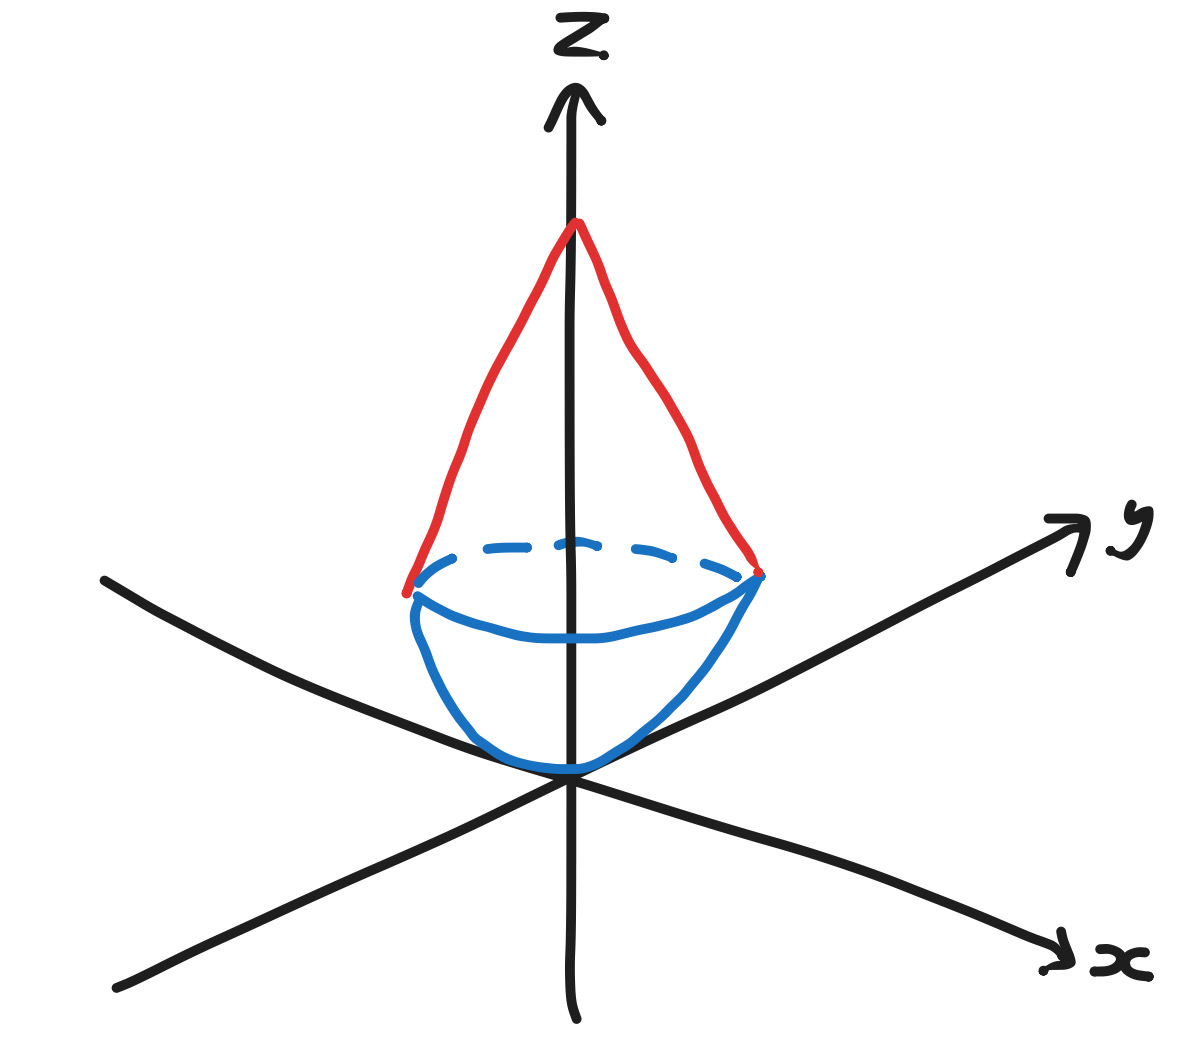
\includegraphics[scale=0.35]{Q3-sketch}
% 	\caption{A sketch of the solid}
% \end{figure}

\begin{align*}
V &= \intlim 0{2\pi} {\intlim 01 {\intlim {r^2}{3-2r} r z} r} \theta\\[1ex]
&= \intlim 0{2\pi} {\intlim 01 {[rz]_{z=r^2}^{3-2r}} r} \theta\\[1ex]
&= \intlim 0{2\pi} {\intlim 01 {r \l( 3 - 2r - r^2 \r)} r} \theta\\[1ex]
&= \intlim 0{2\pi} {\intlim 01 {\l( 3r - 2r^2 - r^3 \r)} r} \theta\\[1ex]
&= \intlim 0{2\pi} {\l[ \f32 r^2 - \f23 r^3 - \f14 r^4 \r]_0^1} \theta\\[1ex]
&= \intlim 0{2\pi} {\l( \f32 - \f23 - \f14 \r)} \theta\\[1ex]
&= \intlim 0{2\pi} {\l( \f{18}{12} - \f8{12} - \f3{12} \r)} \theta\\[1ex]
&= \intlim 0{2\pi} {\f7{12}} \theta\\[1ex]
&= \f{7\pi}6
\end{align*}

\subsection{~}

SciPy gives 3.6651914291880914 with an estimated error of approximately $4.07 \times 10^{-14}$. The actual answer is $\f{7\pi}6 = 3.665191429188092$, so SciPy is correct to 14 decimal places, which also matches the estimated error.

\begin{figure}[h]
	\centering
	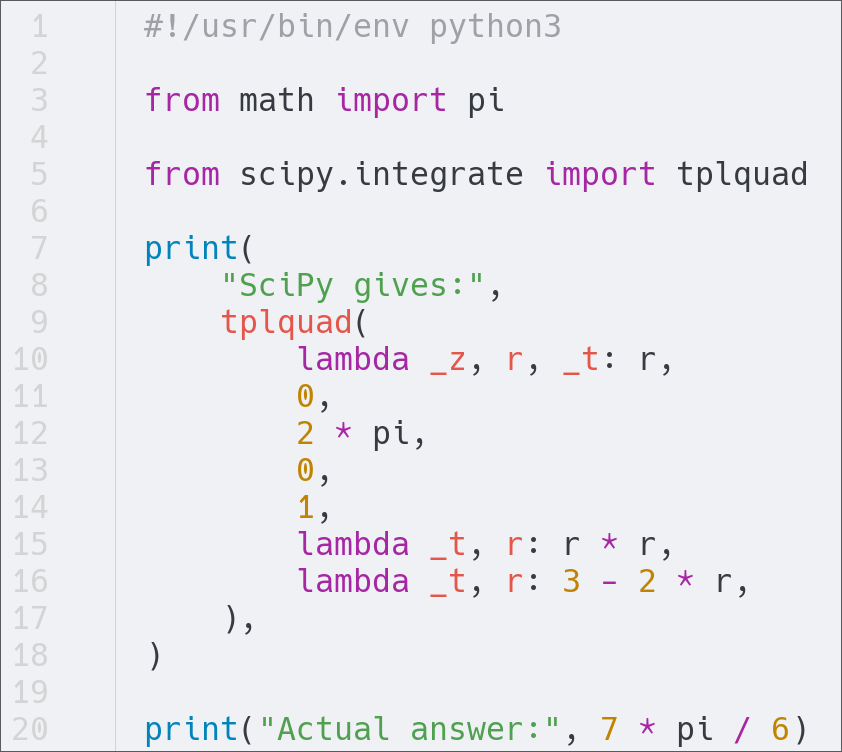
\includegraphics[scale=0.35]{Q3-code}
	\caption{The Python code used to generate this answer}
\end{figure}

%}}}

\end{document}
